\chapter{Modelling a Memory Box}
\label{chap:membox}

What is a memory box?  Figure, why is the example interesting to showcase
metamodelling and model transformations?

What is a model? Metamodel? Instances? Metalevels? Abstractionlevels? Figure
from master thesis.  Always with respect to our concrete example.

Comparison of normal (direct) software development to model-driven software
development, advantages, motivation, product lines, etc

What exactly is model-driven software development?

References to papers, books

\section{A Language Definition Problem?}

What is concrete syntax?  Abstract syntax?  Static semantics?  Dynamic
semantics?  Viewing metamodels as languages, metametamodels as metalanguages,
models as valid words of a certain language.

\section{Static Semantics with Ecore}

Class diagram for memory box, eclass, ereference, Ecore as metametamodel,
epackages, composites, eopposite.

\begin{figure}[!h]
	\centering
  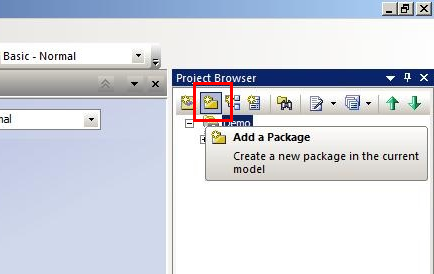
\includegraphics[width=0.7\textwidth]{pics/memBox01.png}
	\caption{memBox01}
	\label{memBox01}
\end{figure}

\begin{figure}[!h]
	\centering
  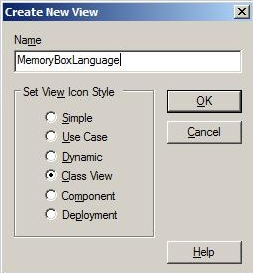
\includegraphics[width=0.7\textwidth]{pics/memBox02.png}
	\caption{memBox02}
	\label{memBox02}
\end{figure}

\begin{figure}[!h]
	\centering
  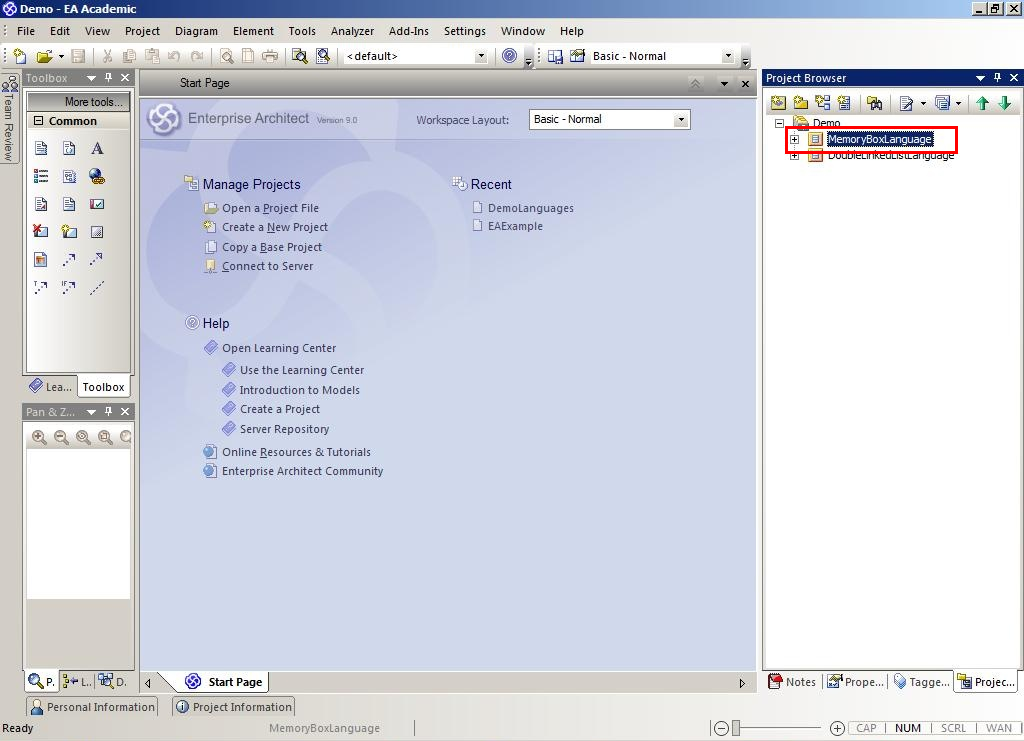
\includegraphics[width=0.7\textwidth]{pics/memBox03.png}
	\caption{memBox03}
	\label{memBox03}
\end{figure}

\begin{figure}[!h]
	\centering
  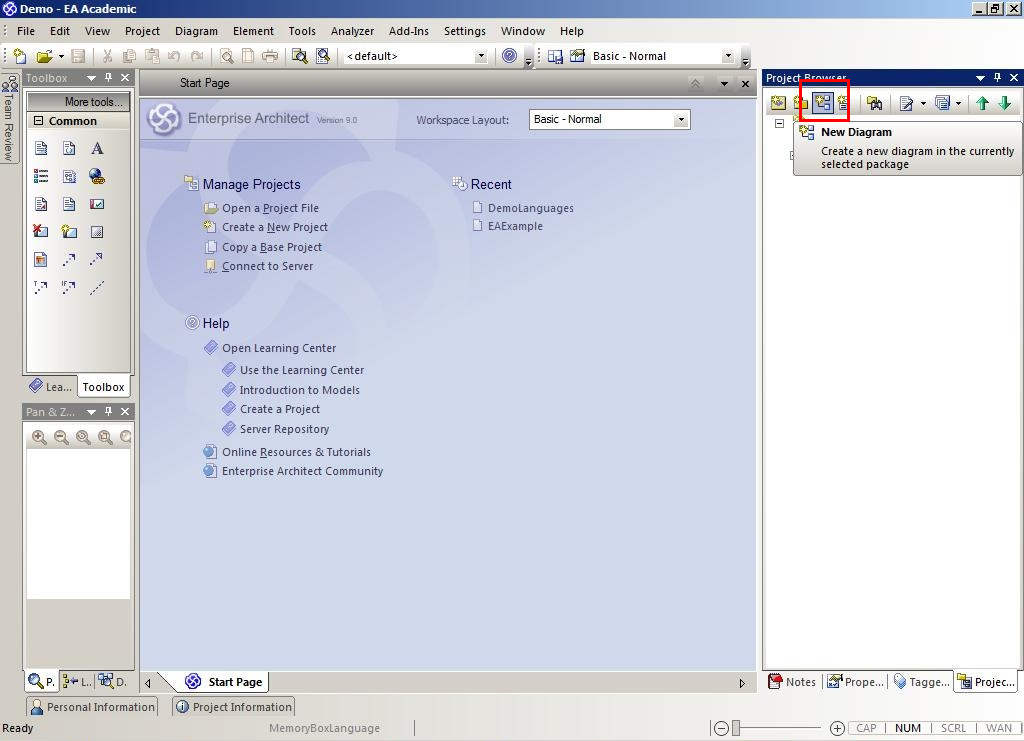
\includegraphics[width=0.7\textwidth]{pics/memBox04.png}
	\caption{memBox04}
	\label{memBox04}
\end{figure}

\begin{figure}[!h]
	\centering
  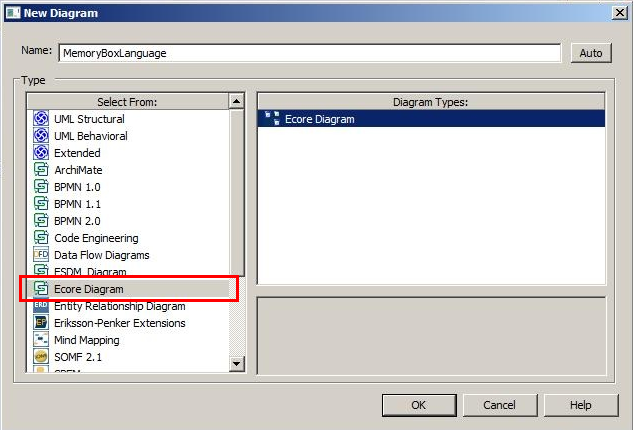
\includegraphics[width=0.7\textwidth]{pics/memBox05.png}
	\caption{memBox05}
	\label{memBox05}
\end{figure}

\begin{figure}[!h]
	\centering
  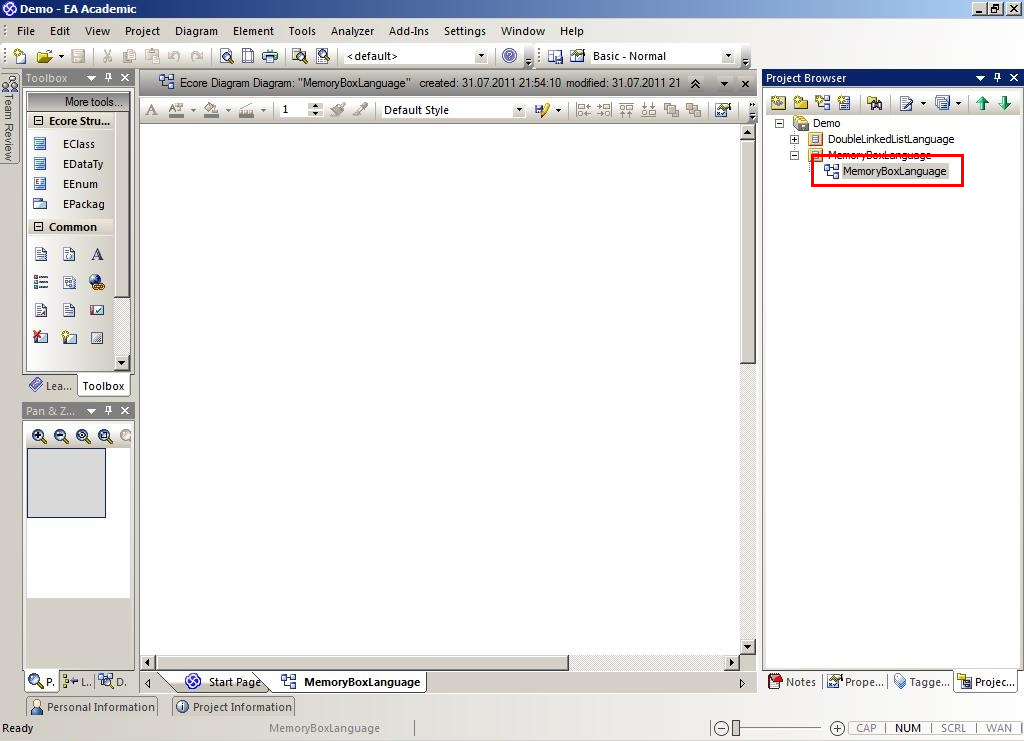
\includegraphics[width=0.7\textwidth]{pics/memBox06.png}
	\caption{memBox06}
	\label{memBox06}
\end{figure}

\begin{figure}[!h]
	\centering
  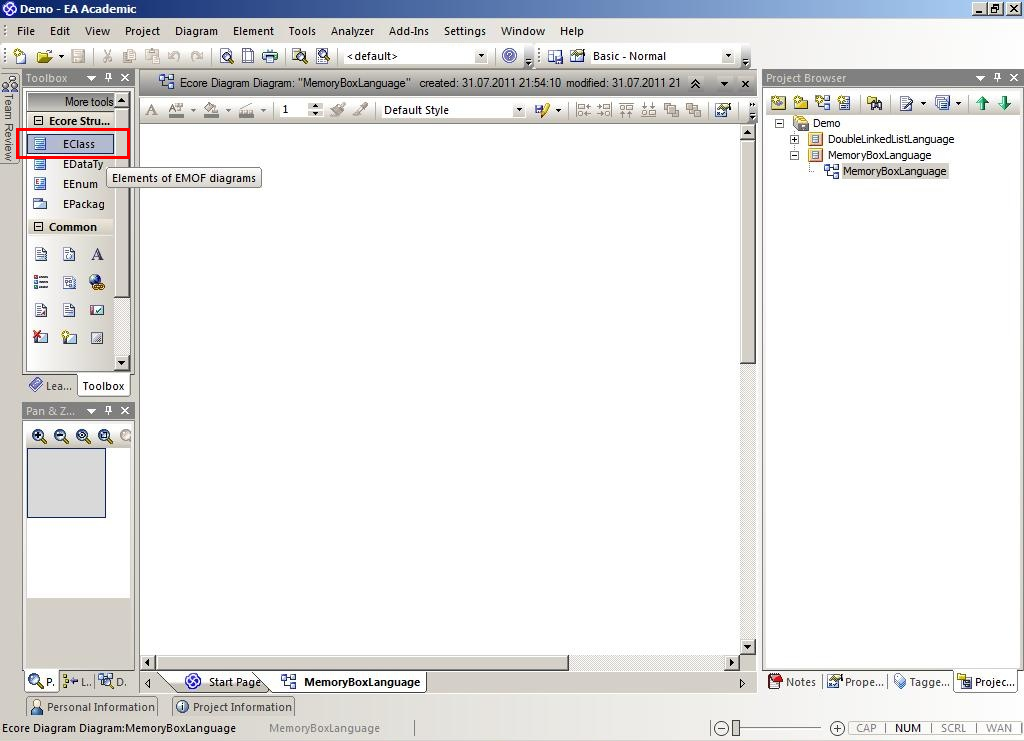
\includegraphics[width=0.7\textwidth]{pics/memBox07.png}
	\caption{memBox07}
	\label{memBox07}
\end{figure}

\begin{figure}[!h]
	\centering
  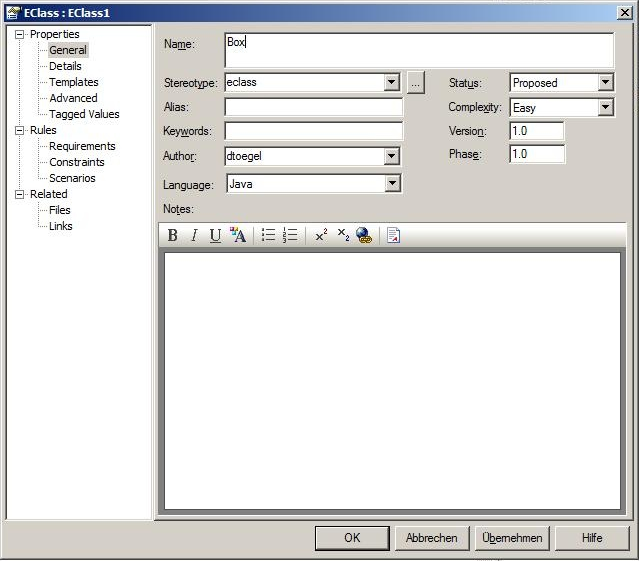
\includegraphics[width=0.7\textwidth]{pics/memBox08.png}
	\caption{memBox08}
	\label{memBox08}
\end{figure}

\begin{figure}[!h]
	\centering
  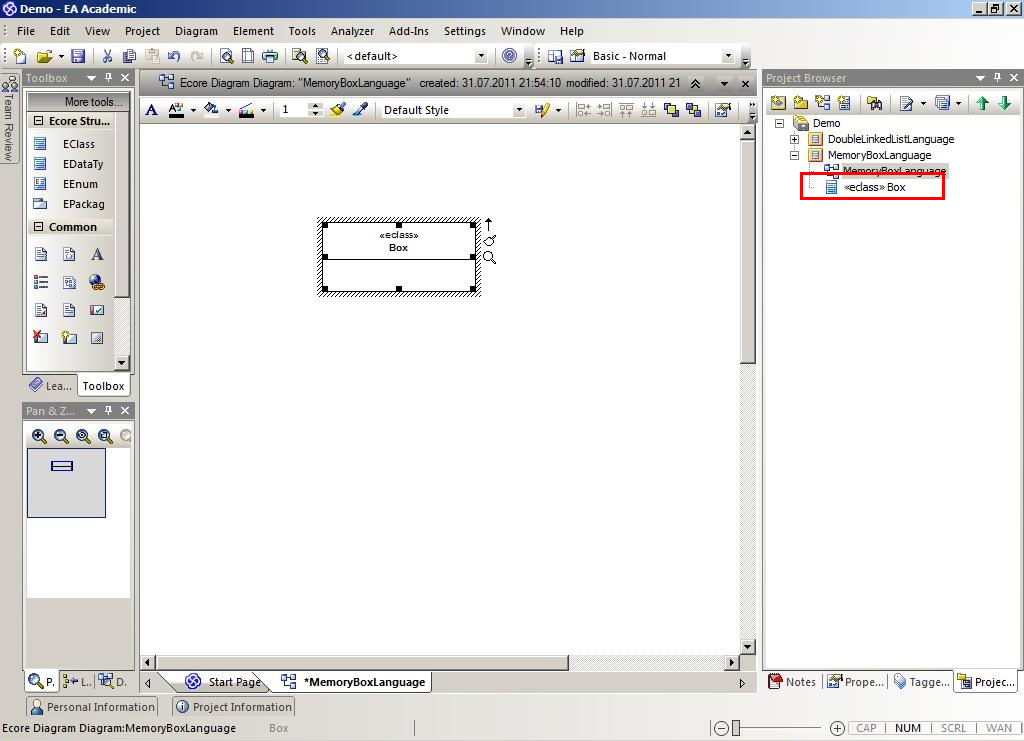
\includegraphics[width=0.7\textwidth]{pics/memBox09.png}
	\caption{memBox09}
	\label{memBox09}
\end{figure}

\begin{figure}[!h]
	\centering
  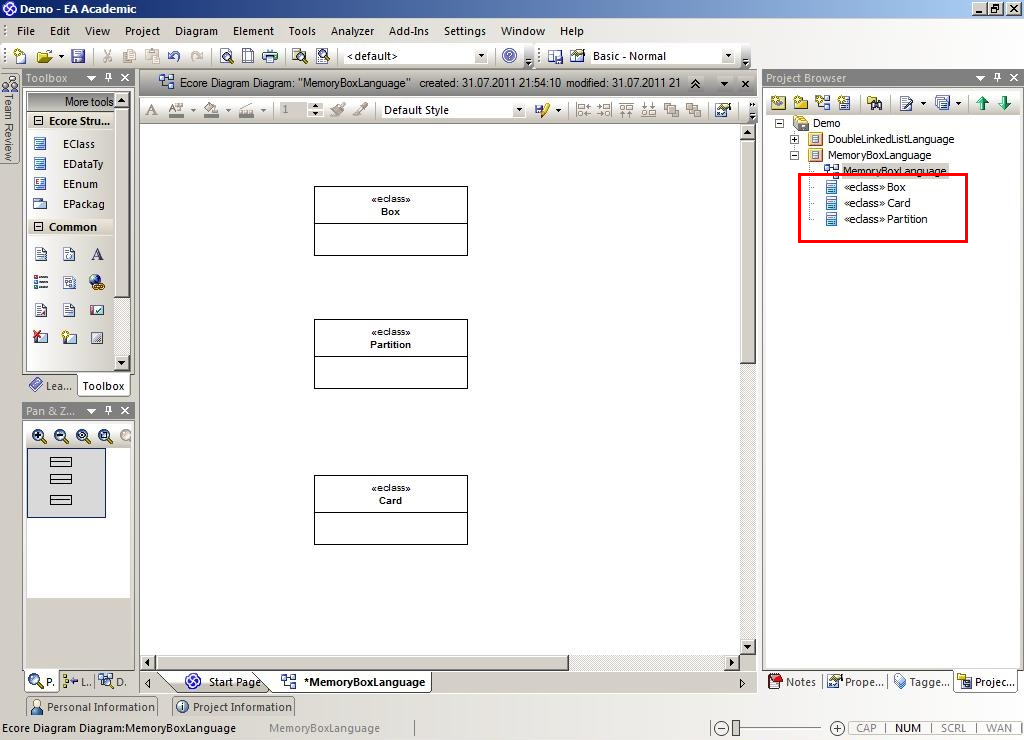
\includegraphics[width=0.7\textwidth]{pics/memBox10.png}
	\caption{memBox10}
	\label{memBox10}
\end{figure}

\begin{figure}[!h]
	\centering
  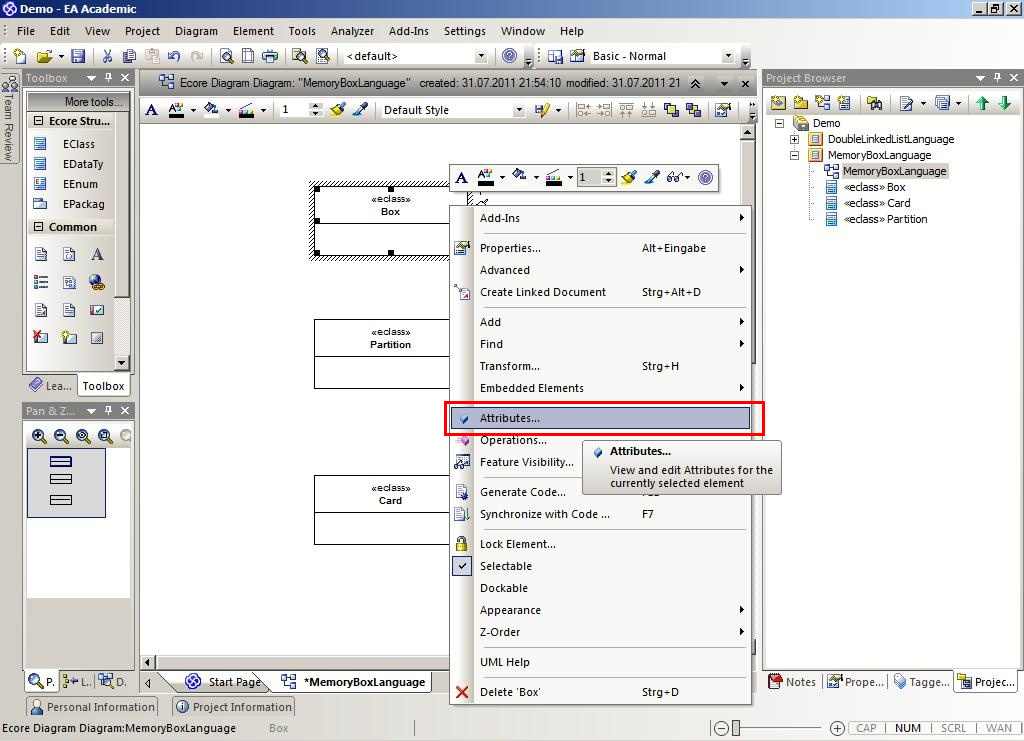
\includegraphics[width=0.7\textwidth]{pics/memBox11.png}
	\caption{memBox11}
	\label{memBox11}
\end{figure}

\begin{figure}[!h]
	\centering
  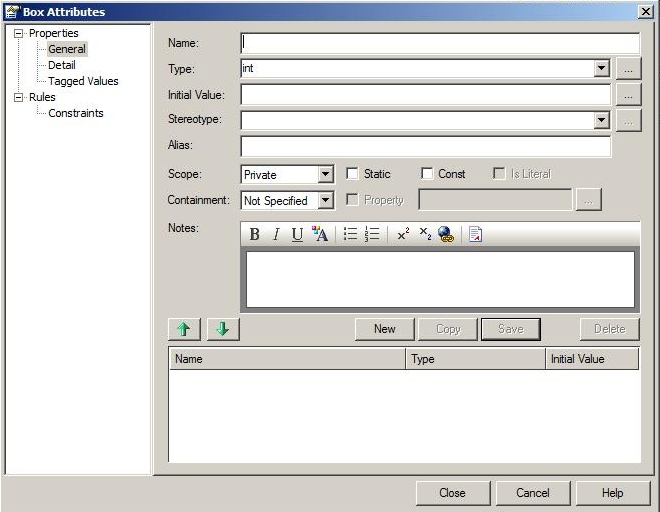
\includegraphics[width=0.7\textwidth]{pics/memBox12.png}
	\caption{memBox12}
	\label{memBox12}
\end{figure}

\begin{figure}[!h]
	\centering
  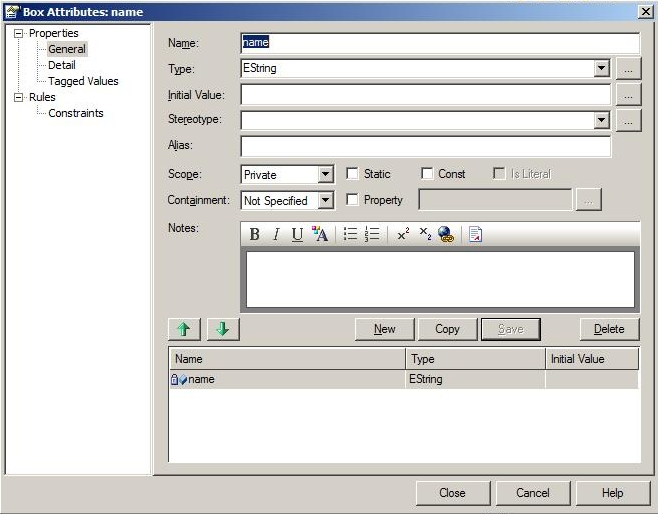
\includegraphics[width=0.7\textwidth]{pics/memBox13.png}
	\caption{memBox13}
	\label{memBox13}
\end{figure}

\begin{figure}[!h]
	\centering
  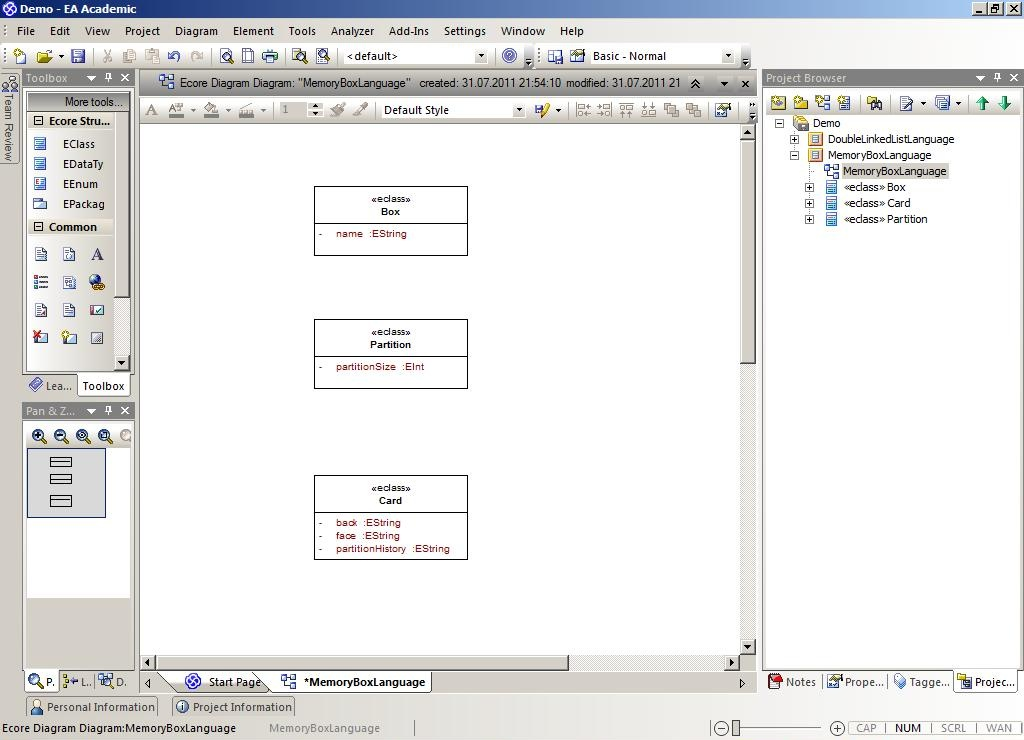
\includegraphics[width=0.7\textwidth]{pics/memBox14.png}
	\caption{memBox14}
	\label{memBox14}
\end{figure}

\begin{figure}[!h]
	\centering
  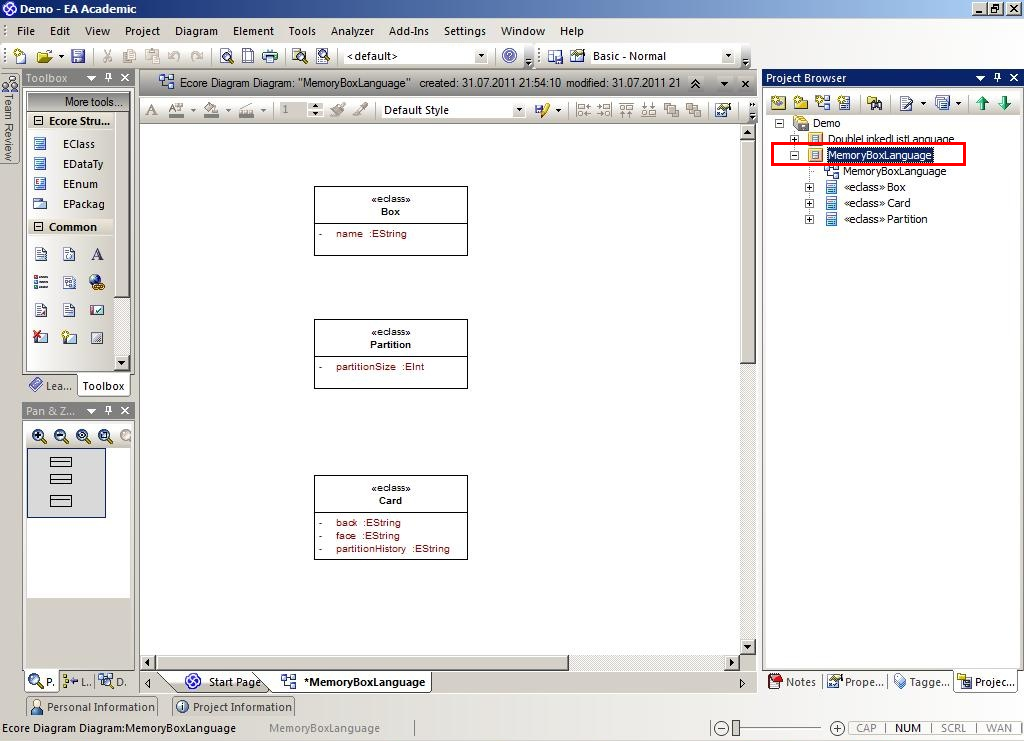
\includegraphics[width=0.7\textwidth]{pics/memBox15.png}
	\caption{memBox15}
	\label{memBox15}
\end{figure}

\begin{figure}[!h]
	\centering
  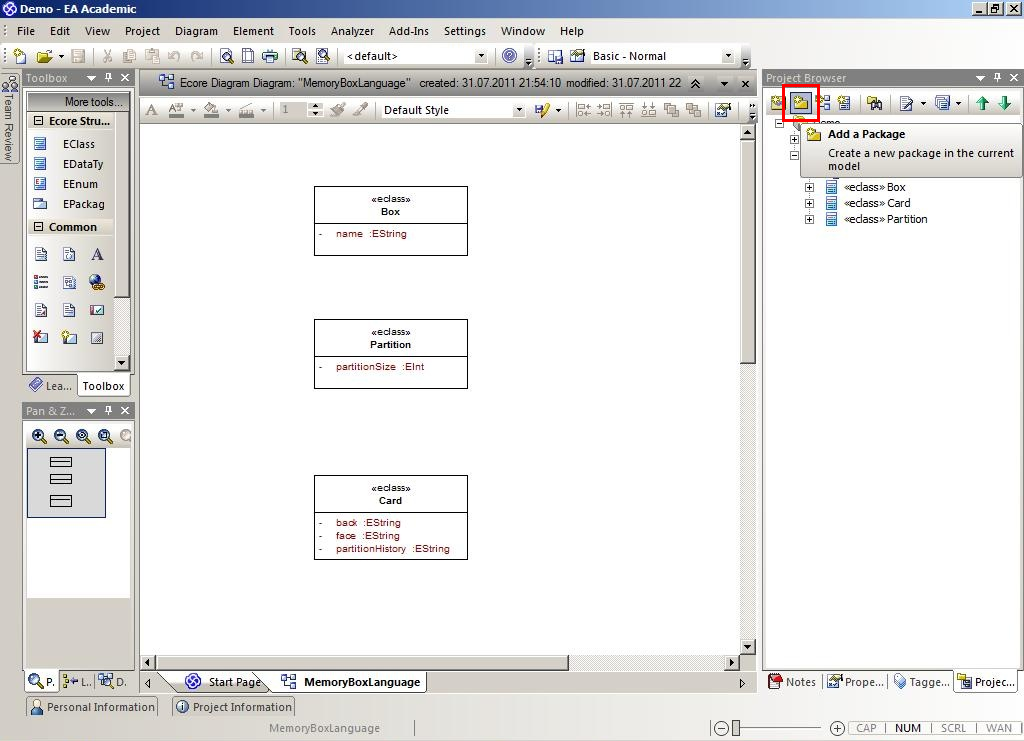
\includegraphics[width=0.7\textwidth]{pics/memBox16.png}
	\caption{memBox16}
	\label{memBox16}
\end{figure}

\begin{figure}[!h]
	\centering
  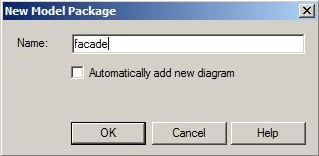
\includegraphics[width=0.7\textwidth]{pics/memBox17.png}
	\caption{memBox17}
	\label{memBox17}
\end{figure}

\begin{figure}[!h]
	\centering
  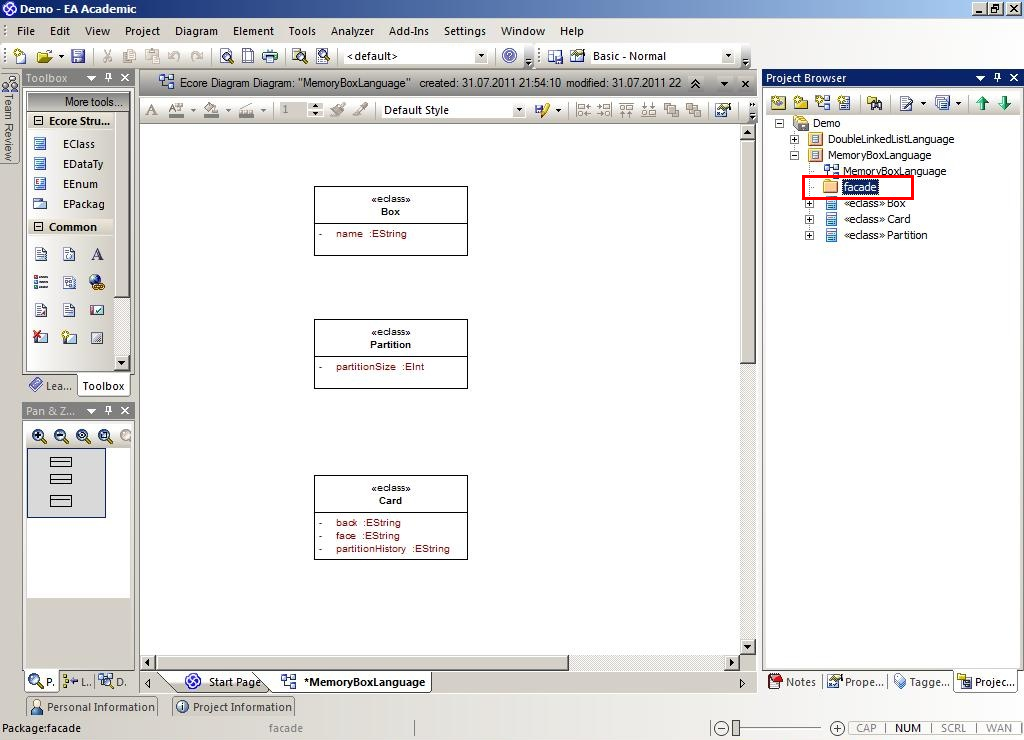
\includegraphics[width=0.7\textwidth]{pics/memBox18.png}
	\caption{memBox18}
	\label{memBox18}
\end{figure}

\begin{figure}[!h]
	\centering
  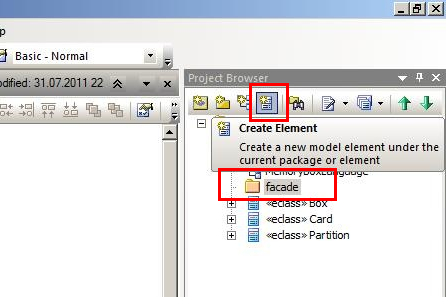
\includegraphics[width=0.7\textwidth]{pics/memBox19.png}
	\caption{memBox19}
	\label{memBox19}
\end{figure}

\begin{figure}[!h]
	\centering
  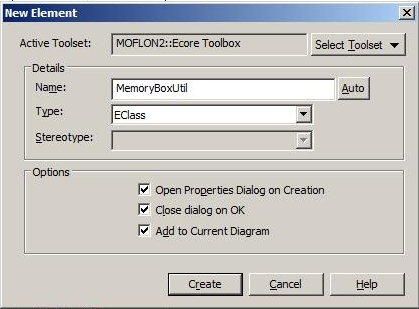
\includegraphics[width=0.7\textwidth]{pics/memBox20.png}
	\caption{memBox20}
	\label{memBox20}
\end{figure}

\begin{figure}[!h]
	\centering
  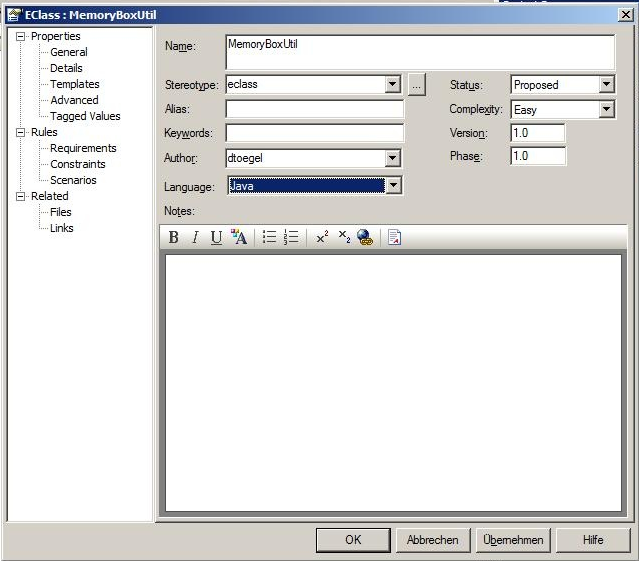
\includegraphics[width=0.7\textwidth]{pics/memBox21.png}
	\caption{memBox21}
	\label{memBox21}
\end{figure}

\begin{figure}[!h]
	\centering
  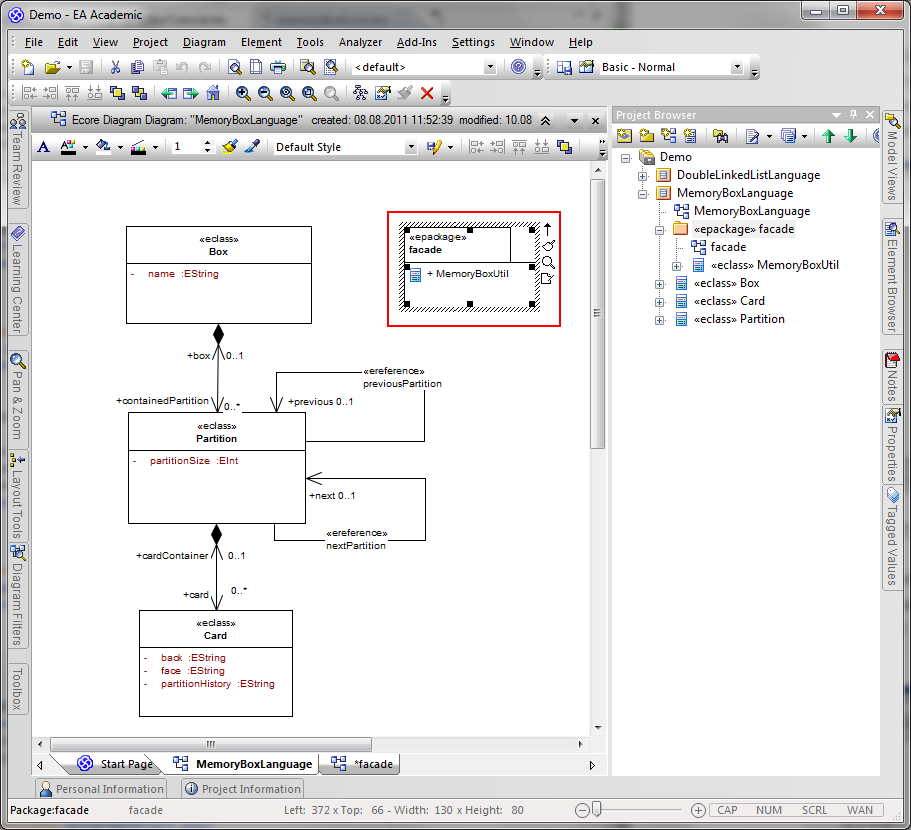
\includegraphics[width=0.7\textwidth]{pics/memBox22.png}
	\caption{memBox22}
	\label{memBox22}
\end{figure}

\begin{figure}[!h]
	\centering
  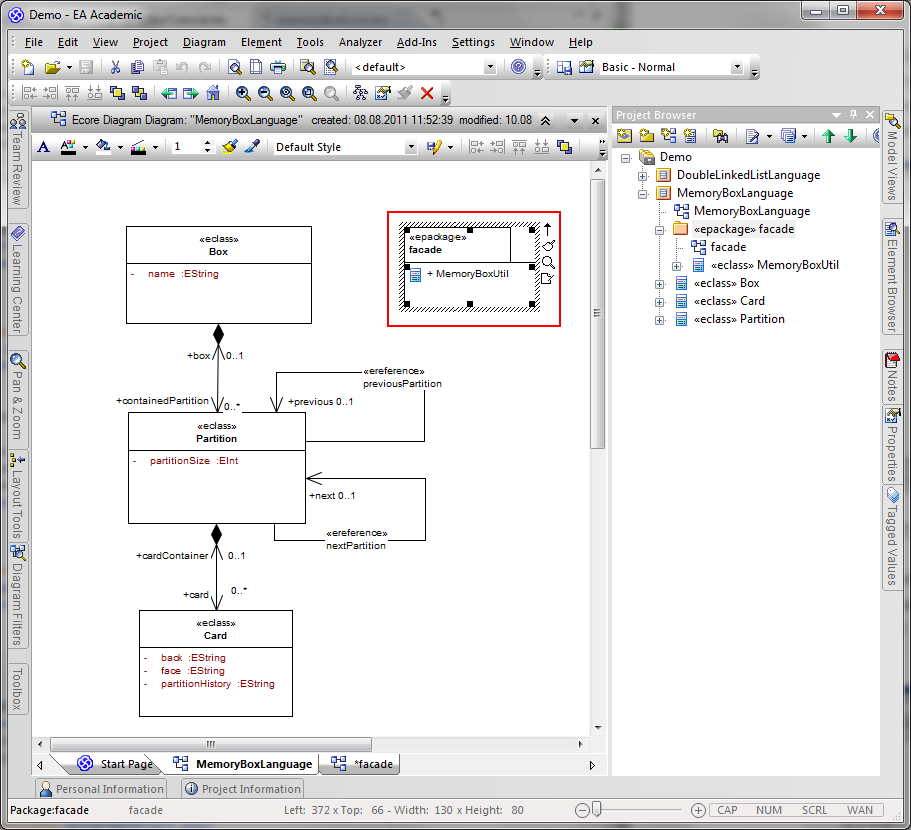
\includegraphics[width=0.7\textwidth]{pics/memBox22.png}
	\caption{memBox22}
	\label{memBox22}
\end{figure}

\begin{figure}[!h]
	\centering
  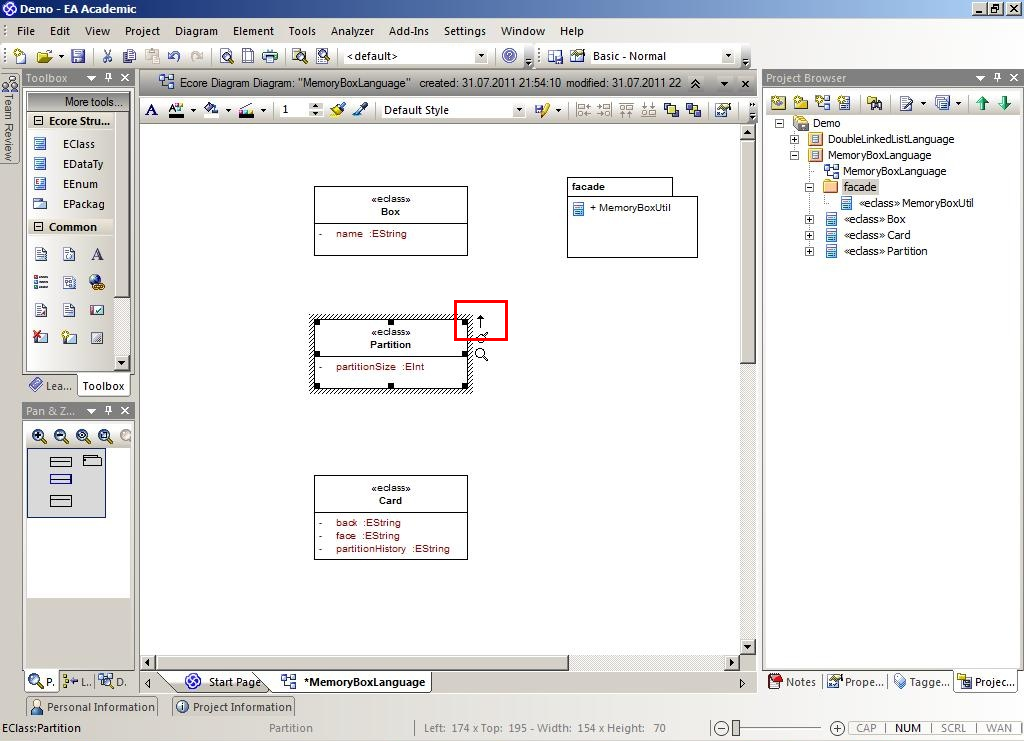
\includegraphics[width=0.7\textwidth]{pics/memBox23.png}
	\caption{memBox23}
	\label{memBox23}
\end{figure}

\begin{figure}[!h]
	\centering
  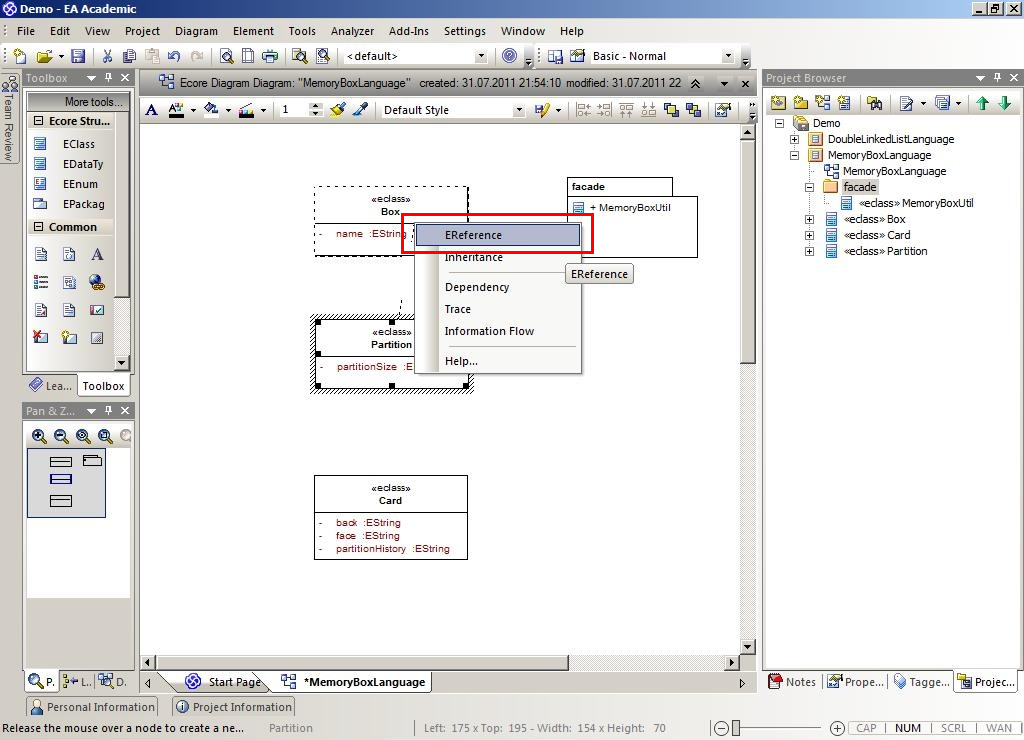
\includegraphics[width=0.7\textwidth]{pics/memBox24.png}
	\caption{memBox24}
	\label{memBox24}
\end{figure}

\begin{figure}[!h]
	\centering
  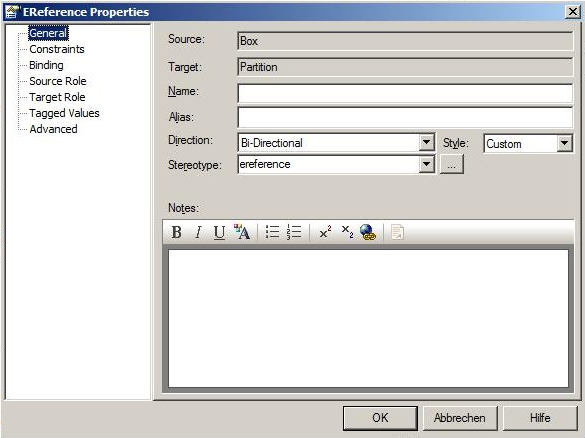
\includegraphics[width=0.7\textwidth]{pics/memBox25.png}
	\caption{memBox25}
	\label{memBox25}
\end{figure}

\begin{figure}[!h]
	\centering
  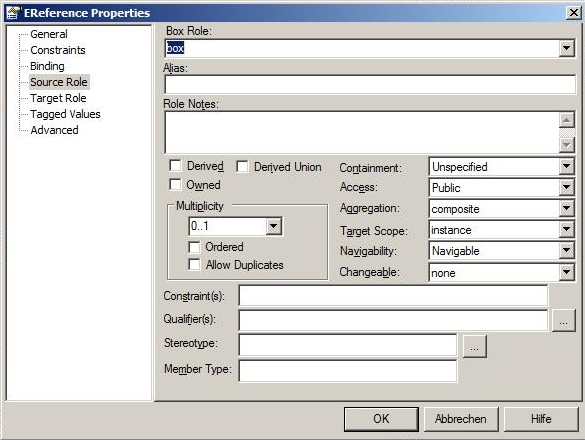
\includegraphics[width=0.7\textwidth]{pics/memBox26.png}
	\caption{memBox26}
	\label{memBox26}
\end{figure}

\begin{figure}[!h]
	\centering
  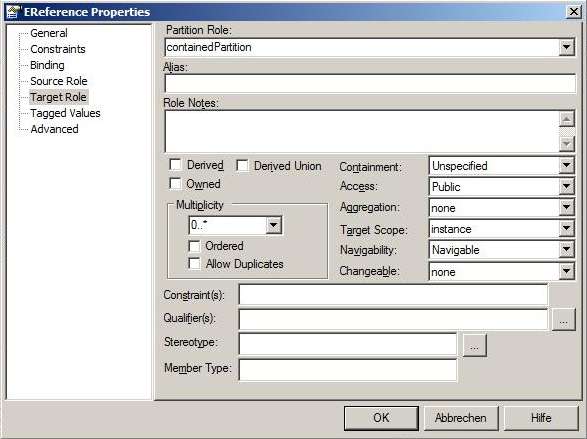
\includegraphics[width=0.7\textwidth]{pics/memBox27.png}
	\caption{memBox27}
	\label{memBox27}
\end{figure}

\begin{figure}[!h]
	\centering
  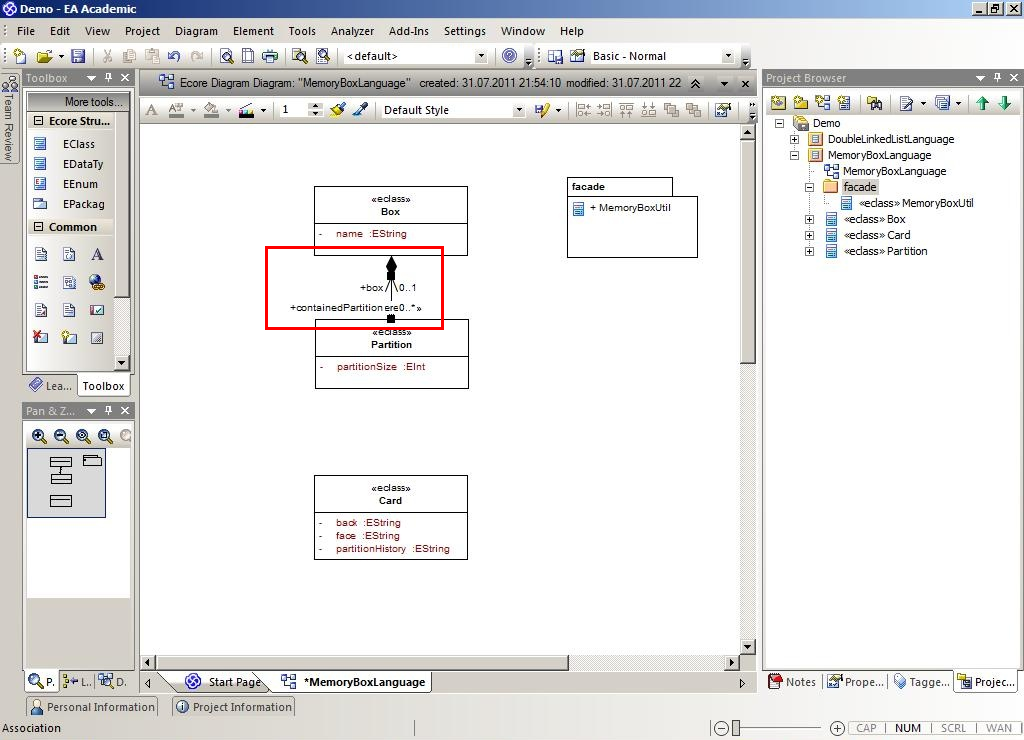
\includegraphics[width=0.7\textwidth]{pics/memBox28.png}
	\caption{memBox28}
	\label{memBox28}
\end{figure}

\begin{figure}[!h]
	\centering
  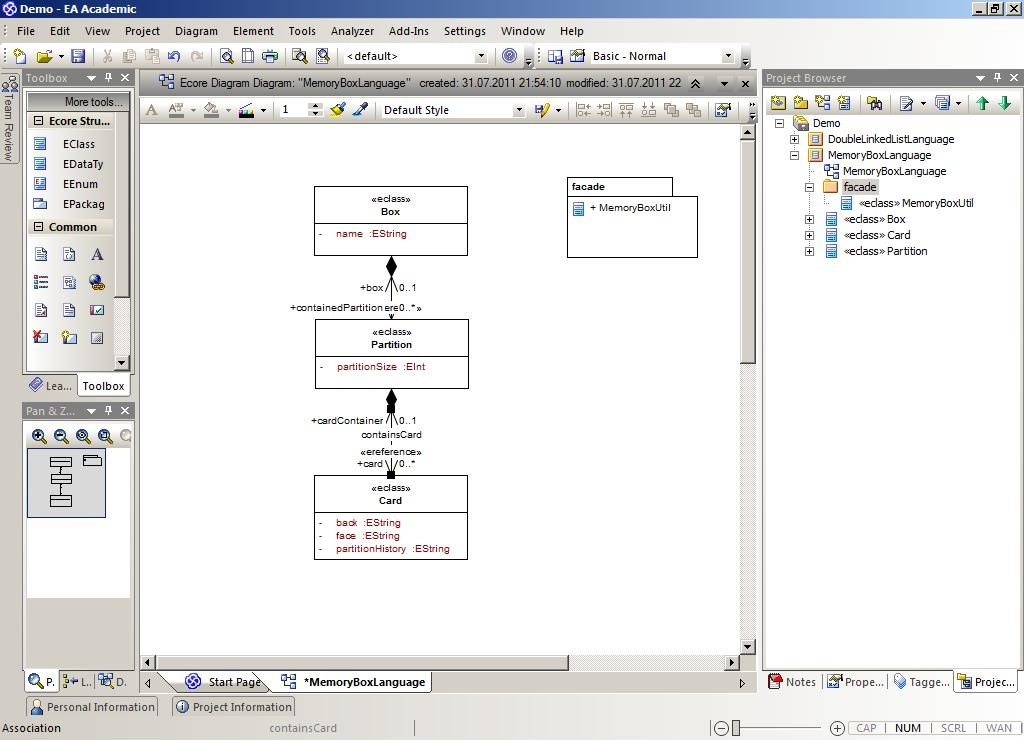
\includegraphics[width=0.7\textwidth]{pics/memBox29.png}
	\caption{memBox29}
	\label{memBox29}
\end{figure}

\begin{figure}[!h]
	\centering
  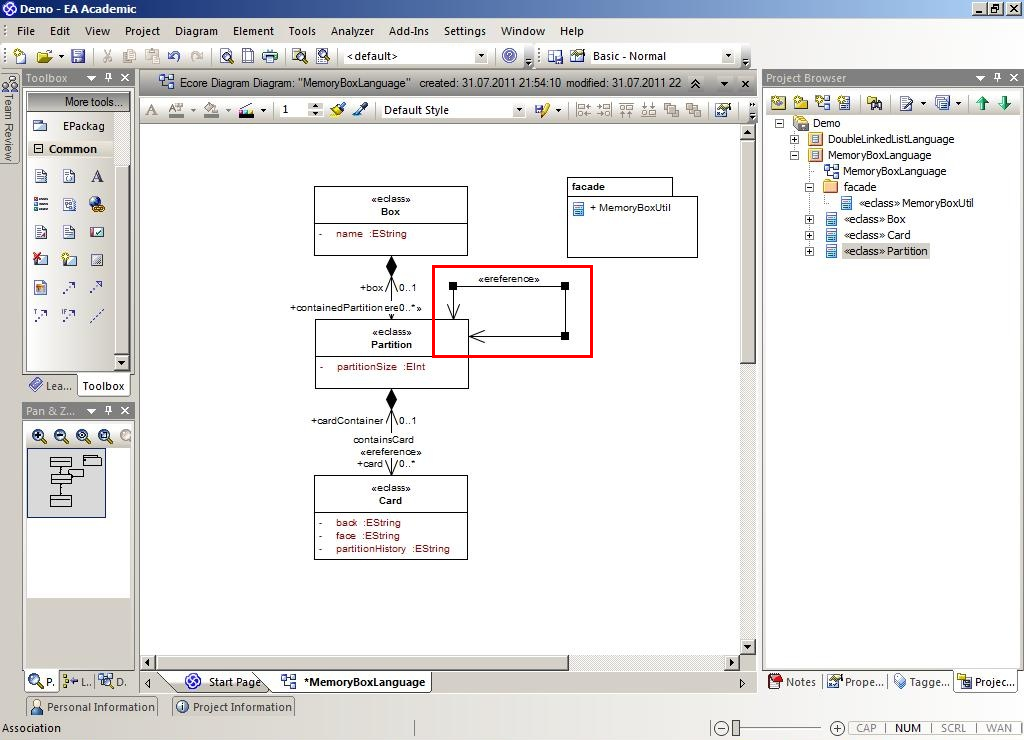
\includegraphics[width=0.7\textwidth]{pics/memBox30.png}
	\caption{memBox30}
	\label{memBox30}
\end{figure}

\begin{figure}[!h]
	\centering
  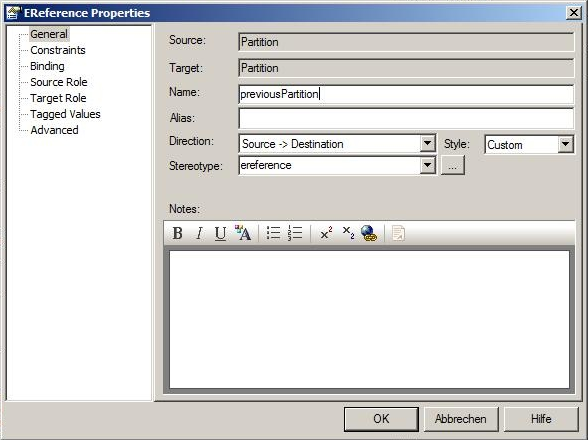
\includegraphics[width=0.7\textwidth]{pics/memBox31.png}
	\caption{memBox31}
	\label{memBox31}
\end{figure}

\begin{figure}[!h]
	\centering
  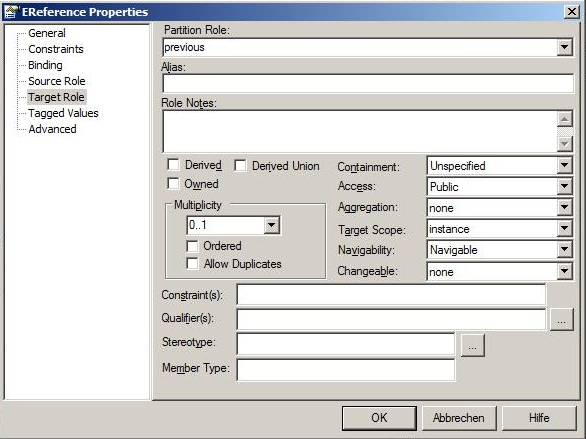
\includegraphics[width=0.7\textwidth]{pics/memBox32.png}
	\caption{memBox32}
	\label{memBox32}
\end{figure}

\begin{figure}[!h]
	\centering
  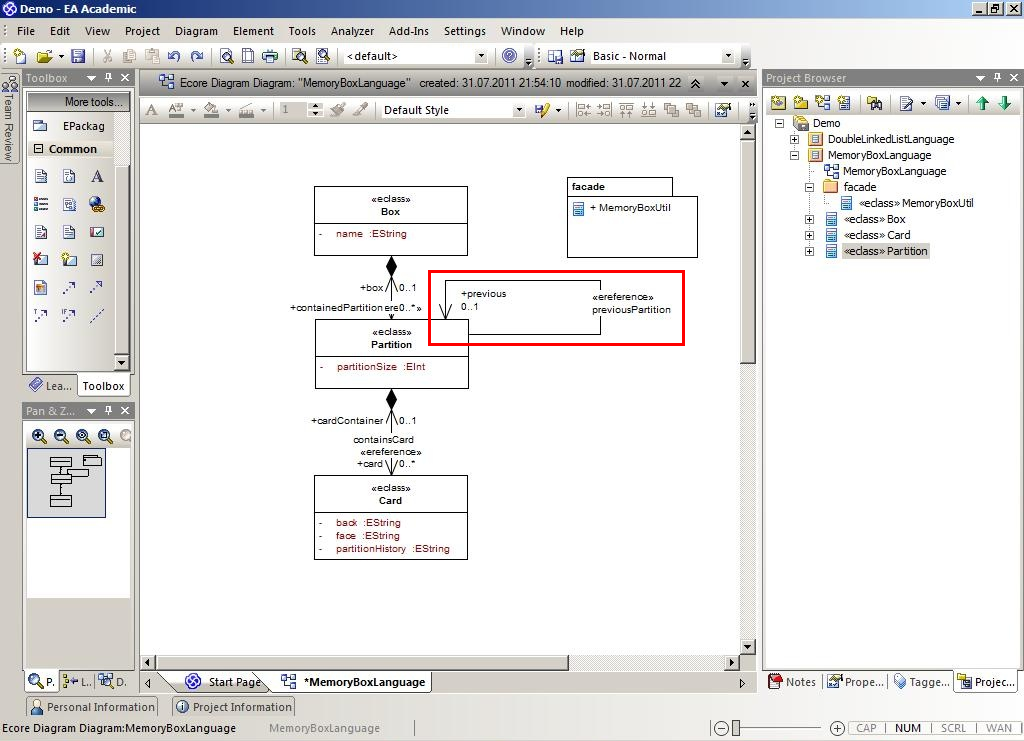
\includegraphics[width=0.7\textwidth]{pics/memBox33.png}
	\caption{memBox33}
	\label{memBox33}
\end{figure}

\begin{figure}[!h]
	\centering
  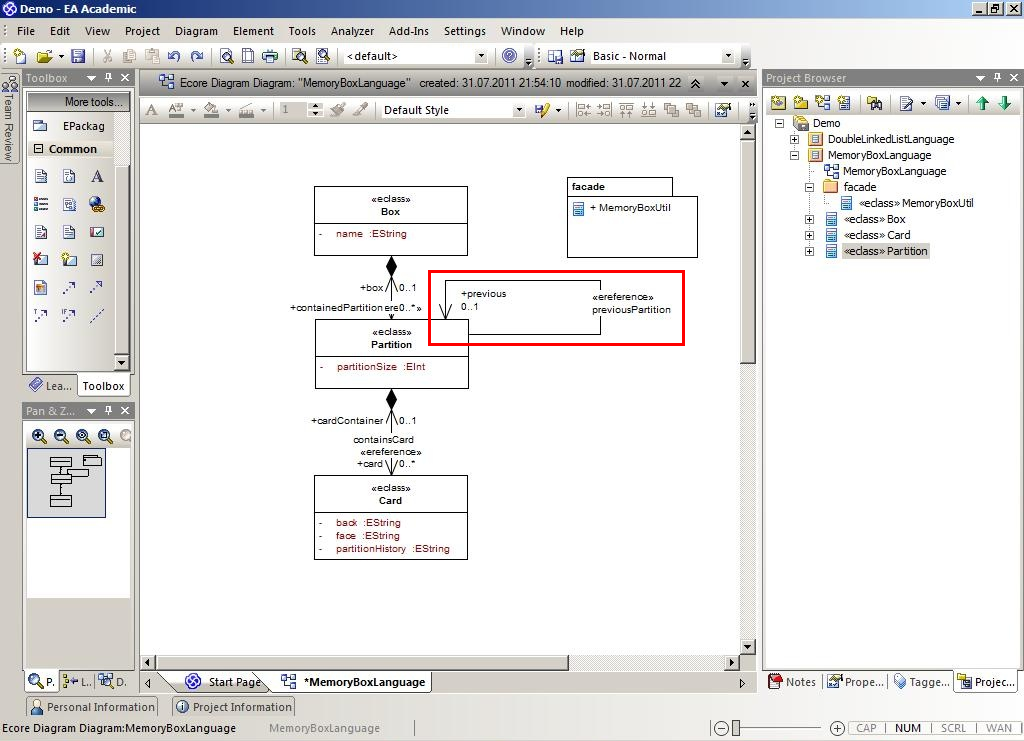
\includegraphics[width=0.7\textwidth]{pics/memBox33.png}
	\caption{memBox33}
	\label{memBox33}
\end{figure}

\begin{figure}[!h]
	\centering
  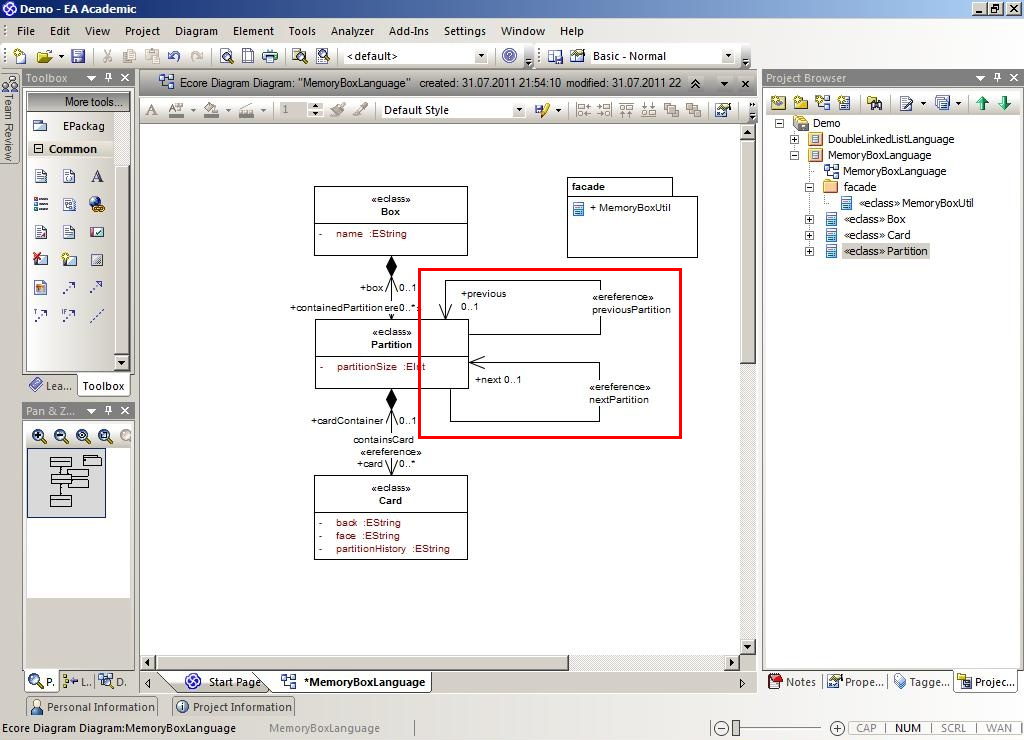
\includegraphics[width=0.7\textwidth]{pics/memBox34.png}
	\caption{memBox34}
	\label{memBox34}
\end{figure}

\begin{figure}[!h]
	\centering
  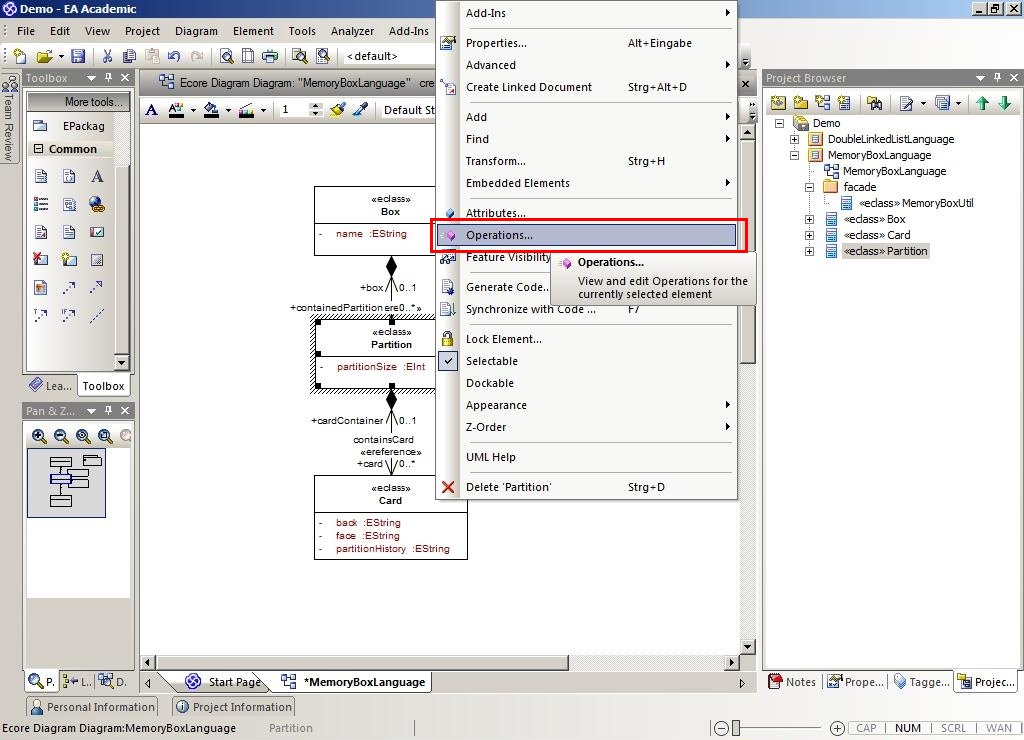
\includegraphics[width=0.7\textwidth]{pics/memBox35.png}
	\caption{memBox35}
	\label{memBox35}
\end{figure}

\begin{figure}[!h]
	\centering
  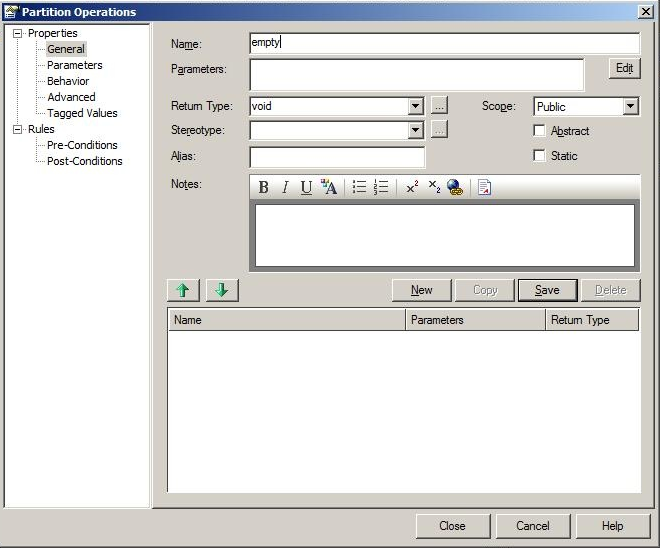
\includegraphics[width=0.7\textwidth]{pics/memBox36.png}
	\caption{memBox36}
	\label{memBox36}
\end{figure}

\begin{figure}[!h]
	\centering
  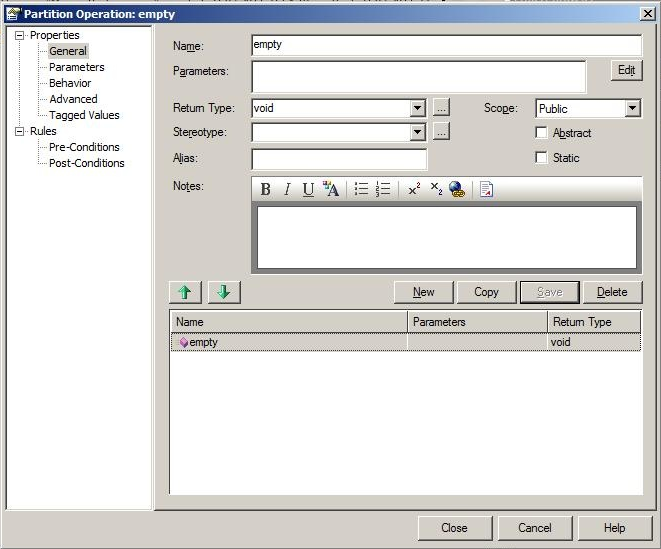
\includegraphics[width=0.7\textwidth]{pics/memBox37.png}
	\caption{memBox37}
	\label{memBox37}
\end{figure}

\begin{figure}[!h]
	\centering
  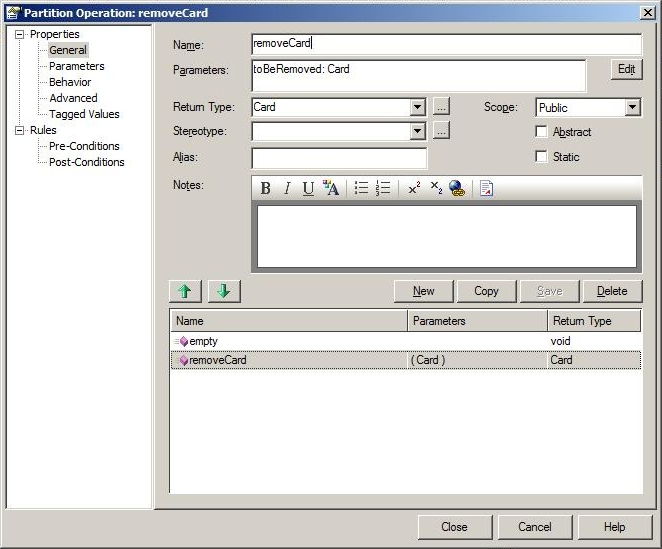
\includegraphics[width=0.7\textwidth]{pics/memBox38.png}
	\caption{memBox38}
	\label{memBox38}
\end{figure}

\begin{figure}[!h]
	\centering
  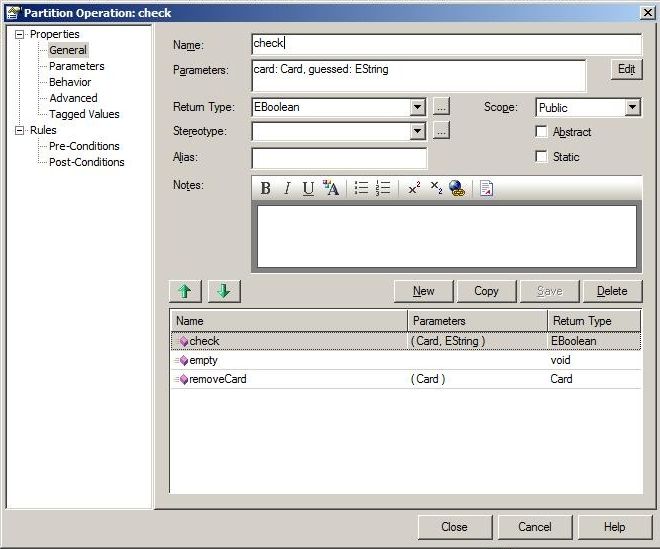
\includegraphics[width=0.7\textwidth]{pics/memBox39.png}
	\caption{memBox39}
	\label{memBox39}
\end{figure}

\begin{figure}[!h]
	\centering
  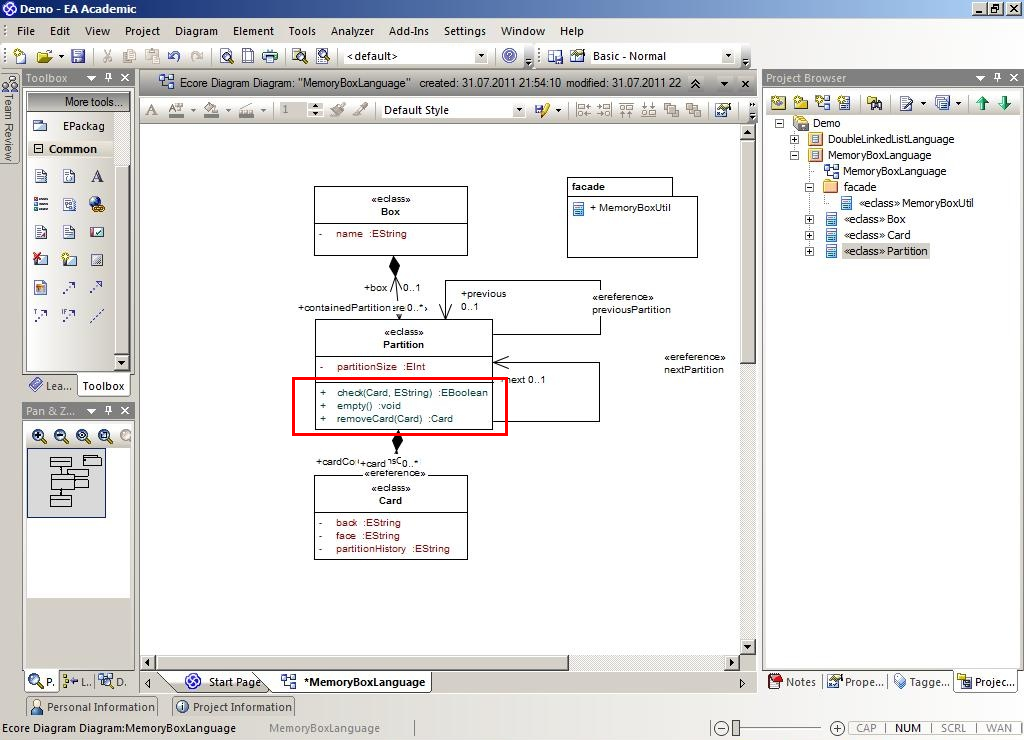
\includegraphics[width=0.7\textwidth]{pics/memBox40.png}
	\caption{memBox40}
	\label{memBox40}
\end{figure}

\begin{figure}[!h]
	\centering
  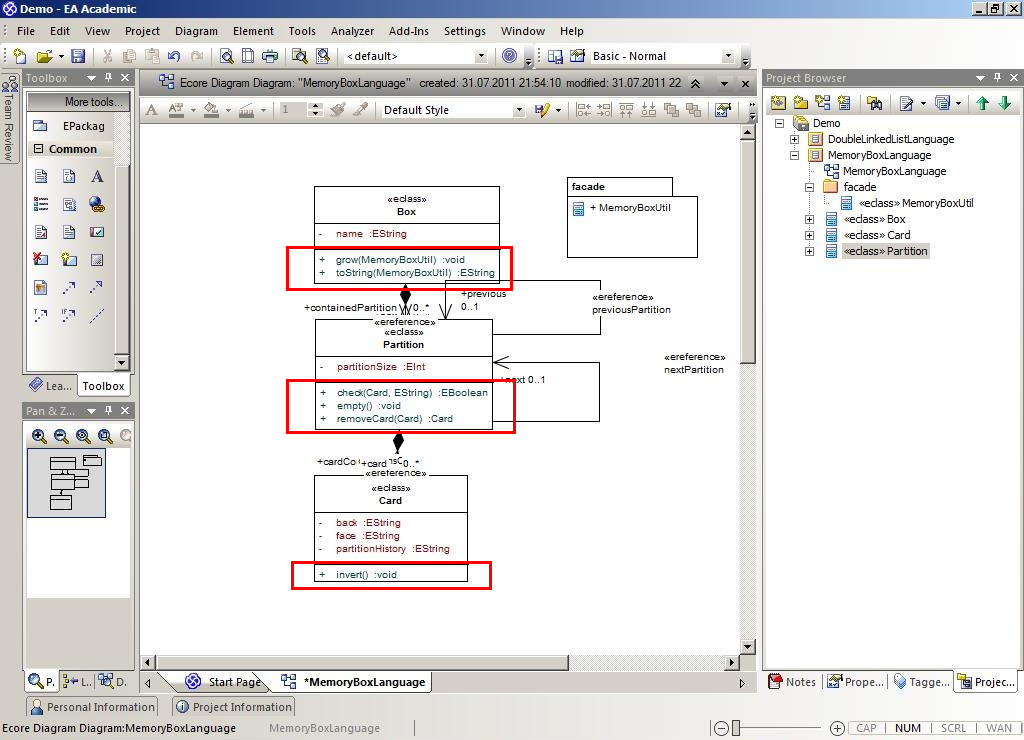
\includegraphics[width=0.7\textwidth]{pics/memBox41.png}
	\caption{memBox41}
	\label{memBox41}
\end{figure}

\begin{figure}[!h]
	\centering
  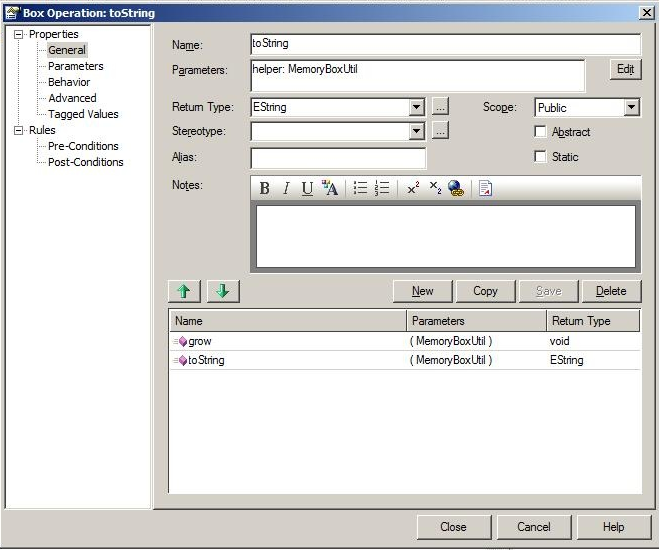
\includegraphics[width=0.7\textwidth]{pics/memBox42.png}
	\caption{memBox42}
	\label{memBox42}
\end{figure}

\begin{figure}[!h]
	\centering
  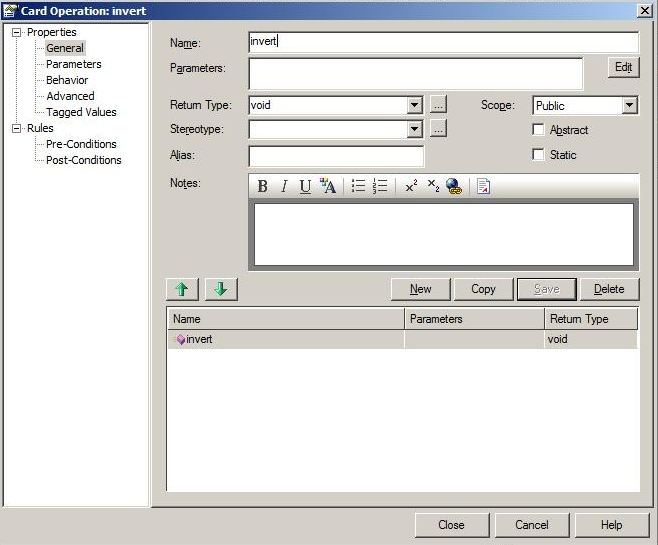
\includegraphics[width=0.7\textwidth]{pics/memBox43.png}
	\caption{memBox43}
	\label{memBox43}
\end{figure}

\begin{figure}[!h]
	\centering
  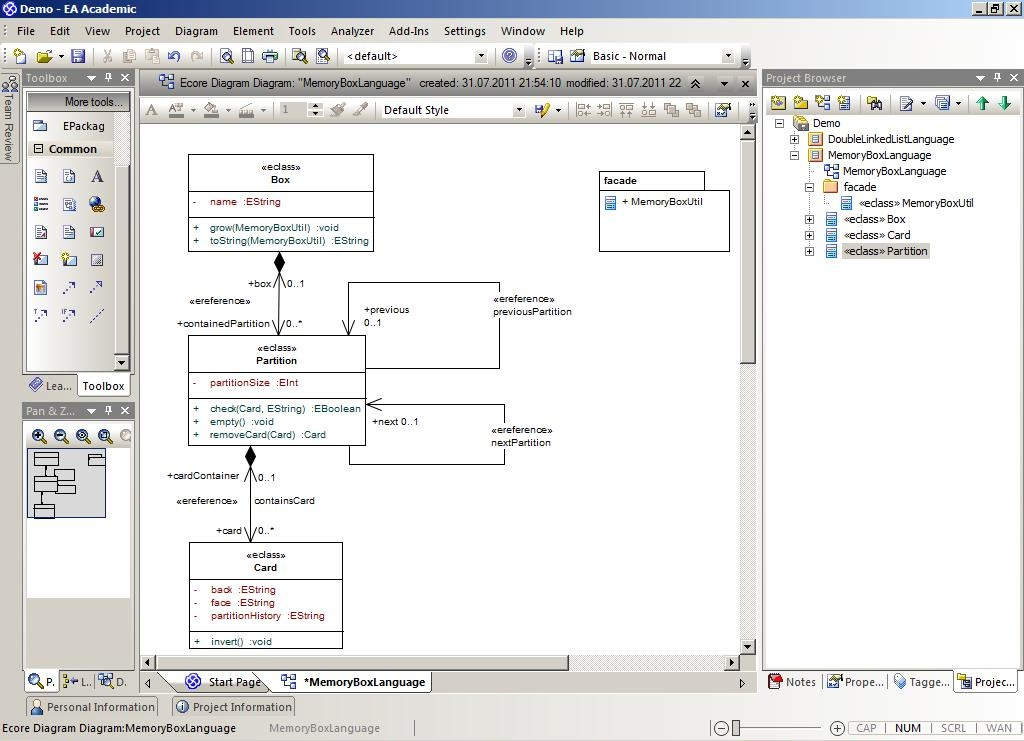
\includegraphics[width=0.7\textwidth]{pics/memBox44.png}
	\caption{memBox44}
	\label{memBox44}
\end{figure}

\section{Dynamic Semantics with SDM}

Graph transformations?  Declarative rules?  Graph grammar?  SDMs?

Based on concrete SDM for memory box:

\subsection*{Activities, Activity Nodes and Edges}

\subsection*{Object and Link Variables}

\subsection*{Expressions}

\subsection*{Statement Nodes}

\subsection*{Start and Stop Nodes}

\subsection*{Attribute Constraints}

\subsection*{Negative Application Conditions}

\subsection*{ForEach Activity Nodes}

\subsection*{Binding Expressions}

\section{Completing the System with a GUI}

Interaction with libraries, frameworks and hand-crafted code.